\documentclass[a4paper,12pt]{article} %размер бумаги устанавливаем А4, шрифт 12пунктов
\usepackage[utf8]{inputenc}
\usepackage{csquotes}
\usepackage[english,russian]{babel}%используем русский и английский языки с переносами
\usepackage{biblatex}
\bibliography{refs}
\usepackage{amssymb,amsfonts,mathtext,enumerate,float} %подключаем нужные пакеты расширений
\usepackage{textcomp}
\usepackage{adjustbox}
\usepackage{graphicx} %хотим вставлять в диплом рисунки?
\makeatletter
\makeatother
\usepackage{sagetex}
\usepackage{geometry} % Меняем поля страницы
\geometry{left=2cm}% левое поле
\geometry{right=1.5cm}% правое поле
\geometry{top=1cm}% верхнее поле
\geometry{bottom=2cm}% нижнее поле
\usepackage{tabularx}
\usepackage{threeparttable}
\usepackage{epstopdf}
\usepackage{amsmath} %отображение математической нотации
\usepackage{caption, subcaption} %подписи}
\usepackage{indentfirst}%отступ вначале параграфа
\usepackage{pscyr}

\captionsetup[table]{labelsep = endash, singlelinecheck=false}
\captionsetup[figure]{name = Рисунок, labelformat=simple, labelsep = endash}

\begin{document}


\newcommand\tline[2]{$\underset{\text{#1}}{\text{\underline{\hspace{#2}}}}$}
\newcommand\nameLine[3]{$\underset{\text{#1}}{\text{\underline{\text{#2}\hspace{#3}}}}$}

\begin{titlepage}
	\centering
	{\fontsize{12pt}{5cm}\selectfont \bfseries Министерство образования и науки Российской Федерации} \\ \vspace{0.5cm}
	{\fontsize{7pt}{5cm}\selectfont ФЕДЕРАЛЬНОЕ ГОСУДАРСТВЕННОЕ АВТОНОМНОЕ ОБРАЗОВАТЕЛЬНОЕ УЧРЕЖДЕНИЕ ВЫСШЕГО ПРОФЕССИОНАЛЬНОГО ОБРАЗОВАНИЯ} \\ 
	\vspace{1cm}
	{\fontsize{12pt}{5cm}\selectfont \bfseries САНКТ-ПЕТЕРБУРГСКИЙ УНИВЕРСИТЕТ ИНФОРМАЦИОННЫХ ТЕХНОЛОГИЙ, МЕХАНИКИ И ОПТИКИ} \\ \vspace{1.5cm}
	
	{\fontsize{14pt}{5cm}\selectfont Кафедра \hspace{1cm} \underline{Систем Управления и Информатики}  \hspace{1cm} Группа \underline{Р3340}} \\
	
	\vspace{2cm}
	
	{\fontsize{20pt}{5cm}\selectfont \bfseries Лабораторная работа №9} \\
	{\fontsize{20pt}{5cm}\selectfont \bfseries “Экспериментальное построение частотных характеристик типовых динамических звеньев”} \\
	\vspace{0.2cm}
	{\fontsize{14pt}{5cm}\selectfont Вариант - 10} \\
	
	\vspace{1.5cm}
	
	\flushleft
	{Выполнилa \hspace{1.8cm} \nameLine{(фамилия, и.о.)}{Ким А. А.}{7cm} (подпись)} \\
	
	\vspace{2cm}
	
	{Проверил \hspace{2cm} \tline{(фамилия, и.о.)}{9cm} (подпись)} \\
	
	\vspace{5cm}
	
	"\underline{\hspace{0.7cm}}"\hspace{0.2cm}\underline{\hspace{2cm}}\hspace{0.2cm}20\underline{\hspace{0.7cm}}г. \hspace{2cm} Санкт-Петербург, \hspace{2cm} 20\underline{\hspace{0.7cm}}г. \\ \vspace{1cm}
	
	Работа выполнена с оценкой \hspace{1cm} \underline{\hspace{8cm}} \\ 
	\vspace{1cm}
	Дата защиты "\underline{\hspace{0.7cm}}"\hspace{0.2cm}\underline{\hspace{2cm}}\hspace{0.2cm}20\underline{\hspace{0.7cm}}г.
\end{titlepage}

\paragraph{Цель работы:}Изучение частотных характеристик типовых динамических звеньев и способов их построения.%*-без нумерации
\paragraph{Исходные данные.}
В данной работе частотные характеристики элементарных динамических звеньев (см. таблицу 1) строятся по точкам на основании данных, полученных экспериментально. В эксперименте исследуется реакция звена на синусоидальное входное воздействие $g(t) = g_m\sin{\omega t}$ с амплитудой входного сигнала $g_m=1$. При заданном значении частоты и амплитуды входного сигнала для определения точек частотной характеристики необходимо измерить значение амплитуды выходного сигнала $y_m$ и сдвиг фаз между входным и выходным сигналом в установившемся режиме $\psi$ (см. рисунок 1). Для определения значения фазы следует учитывать, что на полученных графиках по оси абсцисс отложено время. Значение фазы выходного сигнала в радианах можно рассчитать, используя формулу $\psi=\phi\omega$, где $\omega$ значение частоты входного сигнала в радианах. После соответствующей обработки эти данные дадут одну точку на частотной характеристике. Повторение таких измерений при различных значениях частоты входного сигнала даст массив точек по которым строятся частотные характеристики.
\begin{table}[h!]
	\renewcommand{\arraystretch}{1.8} %строки
	\centering
	\begin{threeparttable}
		\caption{Исходные динамические звенья}
		\begin{tabular}{|c|c|}
			\hline Тип звена & Передаточная функция\\
			\hline Апериодическое 1-го порядка & $W(s) = 
			\displaystyle{\frac{k}{Ts + 1}}$ \\
			\hline Колебательное & $W(s) =
			\displaystyle{\frac{k}{T^2s^2 + 2\xi Ts + 1}}$ \\ 
			\hline Изодромное & $W(s) = \displaystyle{\frac{k(1 + Ts)}{s}}$ \\
			\hline
		\end{tabular}
	\end{threeparttable}
\end{table} 
\par
Параметры исследуемых звеньев: k=4, T=0.8, $\xi$=0.45
\par
Сопрягающая частота $\frac{1}{T}=1.25c^{-1}$
\begin{figure}[H]
	\centering
	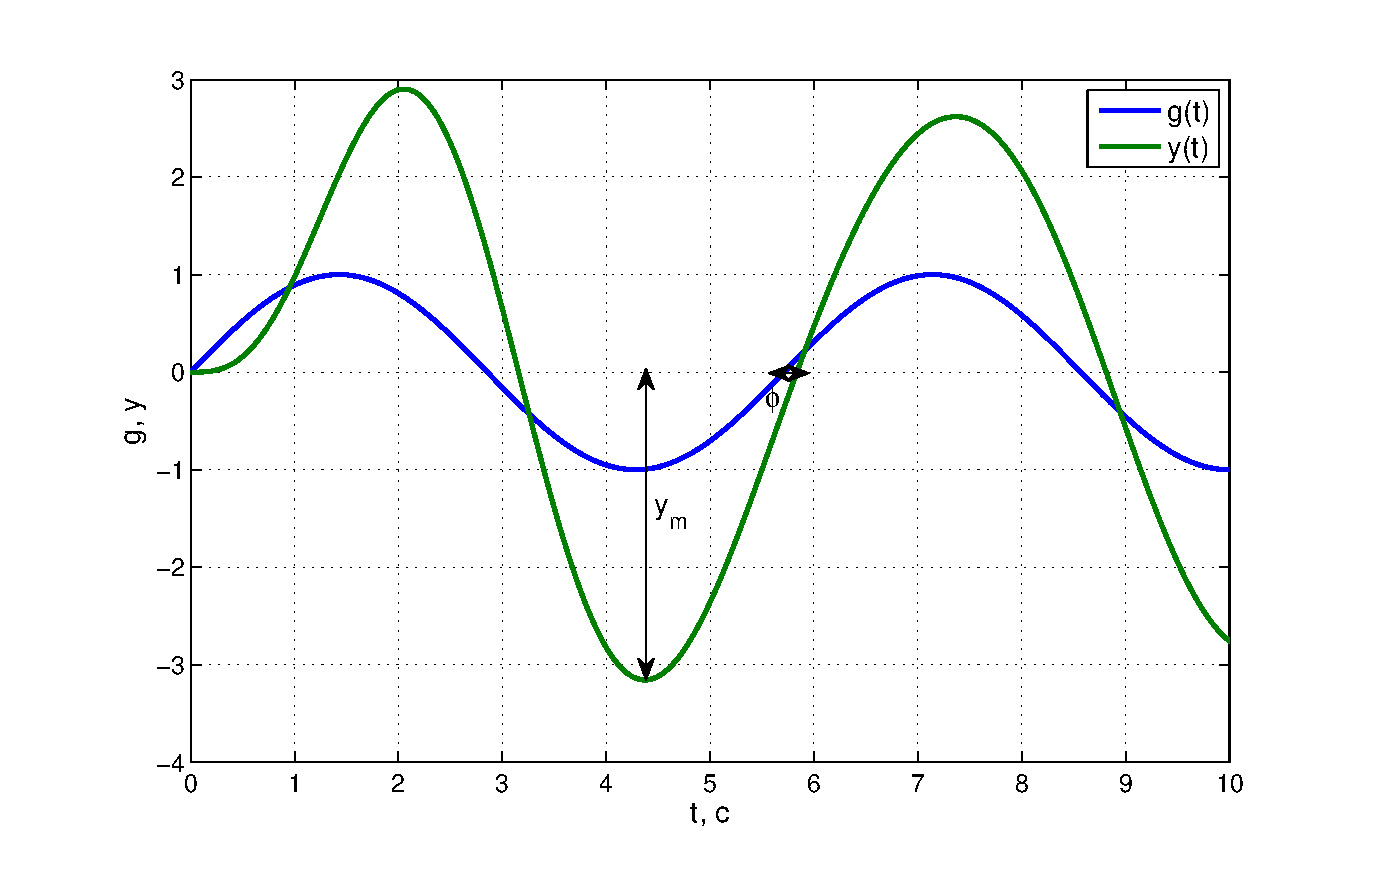
\includegraphics[width=0.8\linewidth]{scheme/timedia.eps}
	\caption{Временная диаграмма}
\end{figure}

\newpage
\begin{center}
\section{Апериодическое звено 1-го порядка}
\end{center}

В таблице 2 представлены данные при исследовании апериодического звена 1-го порядка.
\begin{table}[h!]
	\renewcommand{\arraystretch}{1.8} %строки
	\centering
	\begin{threeparttable}
		\caption{Экспериментальные данные для апериодического звена 1-го порядка}
		\begin{tabular}{|c|c|c|c|c|}
			\hline $\omega$, рад/с & $lg\omega$ & $A(\omega)$ & $L(\omega)=20lgA(\omega)$ & $\psi(\omega)$, град\\
			\hline 0,125 & -0,90 & 9,95 & 19,95 & -5,37\\
			\hline 0,175 & -0,75 & 9,90 & 19,91 & -7,40\\
			\hline 0,225 & -0,64 & 9,84 & 19,86 & -10,91\\
			\hline 0,275 & -0,56 & 9,76 & 19,79 & -12,85\\
			\hline 0,325 & -0,48 & 9,68 & 19,71 & -15,13\\
			\hline 0,375 & 0,42 & 9,58 & 19,63 & -15,89\\
			\hline 0,425 & 0,37 & 9,47 & 19,53 & -18,60\\
			\hline 0,475 & 0,32 & 9,36 & 19,43 & -20,84\\
			\hline 0,500 & 0,30 & 9,31 & 19,37 & -22,43\\
			\hline 1,000 & 0,0 & 8,11 & 18,18 & -36,78\\
			\hline 2,000 & 0,30 & 6,22 & 15,88 & -53,05\\
			\hline 3,000 & 0,47 & 5,00 & 13,99 & -61,02\\
			\hline 4,000 & 0,60 & 4,17 & 12,41 & -65,77\\
			\hline 5,000 & 0,69 & 3,58 & 11,08 & -70,19\\
			\hline 7,000 & 0,84 & 2,78 & 8,90 & -74,20\\
			\hline 10,000 & 1,00 & 2,08 & 6,39 & -77,35\\			
			\hline 20,000 & 1,30 & 1,137 & 1,11 & -87,09\\			
			\hline 60,000 & 1,77 & 0,40 & -7,89 & -89,38\\			
			\hline
		\end{tabular}
	\end{threeparttable}
\end{table}

На рисунках 2-7 представлены частотные характеристики апериодического звена 1-го порядка.
\begin{figure}[H]
	\centering
	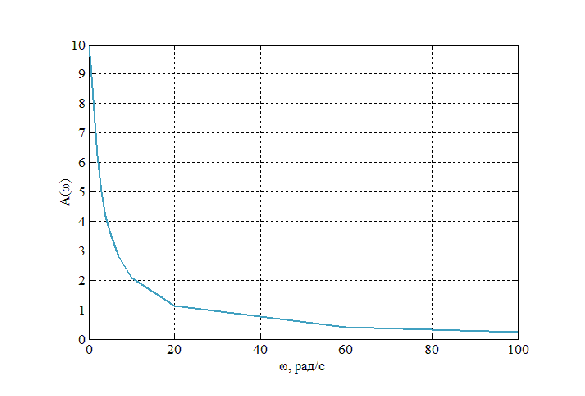
\includegraphics[width=1\linewidth]{scheme/Ach1.eps}
	\caption{АЧХ}
\end{figure}
\begin{figure}[H]
	\centering
	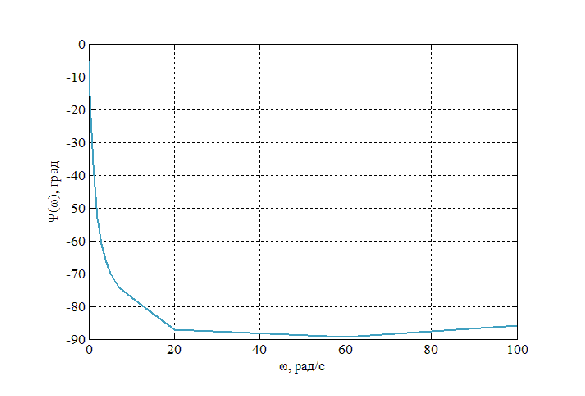
\includegraphics[width=1\linewidth]{scheme/Fch1.eps}
	\caption{ФЧХ}
\end{figure}
\begin{figure}[H]
	\centering
	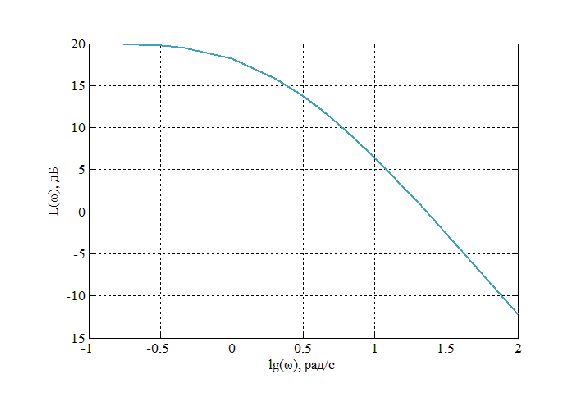
\includegraphics[width=1\linewidth]{scheme/Lach1.eps}
	\caption{ЛАЧХ}
\end{figure}
\begin{figure}[H]
	\centering
	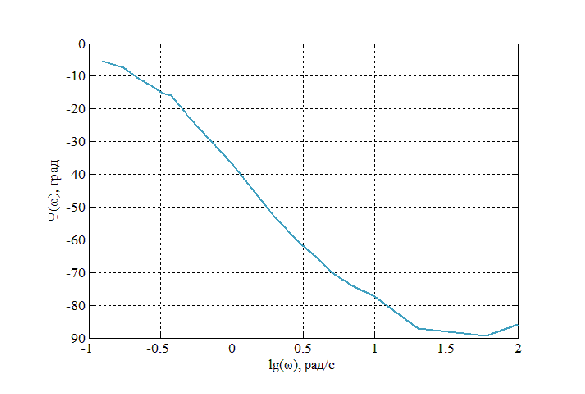
\includegraphics[width=1\linewidth]{scheme/Lfch1.eps}
	\caption{ЛФЧХ}
\end{figure}
\begin{figure}[H]
	\centering
	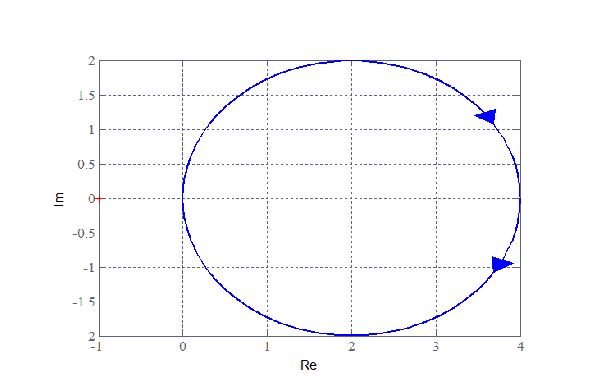
\includegraphics[width=1\linewidth]{scheme/Afch1.eps}
	\caption{АФЧХ}
\end{figure}
\begin{figure}[H]
	\centering
	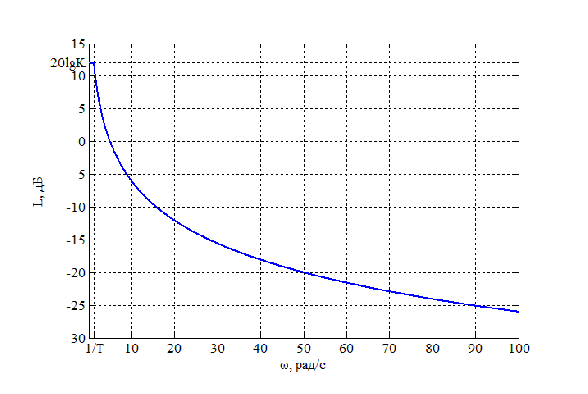
\includegraphics[width=1\linewidth]{scheme/Asi1.eps}
	\caption{Асимптотическая ЛАЧХ}
\end{figure}

\newpage
\begin{center}
\section{Колебательное звено}
\end{center}

В таблице 3 представлены данные при исследовании колебательного звена.
\begin{table}[h!]
	\renewcommand{\arraystretch}{1.8} %строки
	\centering
	\begin{threeparttable}
	\caption{Экспериментальные данные для колебательного звена}
	\begin{tabular}{|c|c|c|c|c|}
		\hline $\omega$, рад/с & $lg\omega$ & $A(\omega)$ & $L(\omega)=20lgA(\omega)$ & $\psi(\omega)$, град\\
		\hline 0,125 & -0,90 & 4,02 & 12,09 & -4,81\\
		\hline 0,175 & -0,75 & 4,04 & 12,14 & -6,67\\
		\hline 0,225 & -0,64 & 4,06 & 12,18 & -9,98\\
		\hline 0,275 & -0,56 & 4,11 & 12,29 & -10,61\\
		\hline 0,325 & -0,48 & 4,20 & 12,48 & -13,65\\
		\hline 0,375 & 0,42 & 4,30 & 12,66 & -14,18\\
		\hline 0,425 & 0,37 & 4,37 & 12,81 & -21,16\\
		\hline 0,475 & 0,32 & 4,41 & 12,90 & -26,92\\
		\hline 0,500 & 0,30 & 4,43 & 12,93 & -27,36\\
		\hline 1,000 & 0,00 & 4,01 & 12,07 & -67,72\\
		\hline 2,000 & 0,30 & 2,59 & 8,26 & -114,36\\
		\hline 3,000 & 0,47 & 1,70 & 4,62 & -140,95\\
		\hline 4,000 & 0,60 & 1,18 & 1,48 & -155,61\\
		\hline 5,000 & 0,69 & 0,88 & -1,05 & -164,73\\
		\hline 7,000 & 0,84 & 0,51 & -5,68 & -179,28\\				
		\hline
	\end{tabular}
	\end{threeparttable}
\end{table}

На рисунках 8-13 представлены частотные характеристики колебательного звена.
\begin{figure}[H]
	\centering
	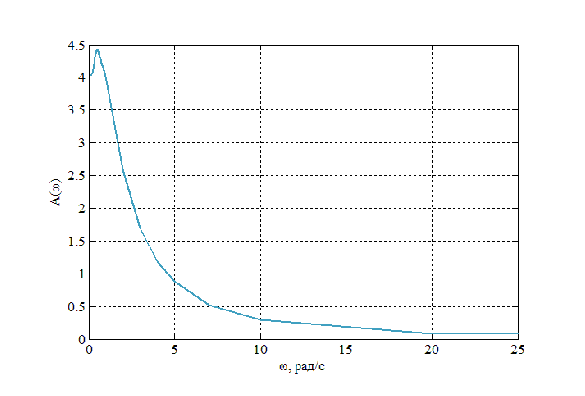
\includegraphics[width=1\linewidth]{scheme/Ach2.eps}
	\caption{АЧХ}
\end{figure}
\begin{figure}[H]
	\centering
	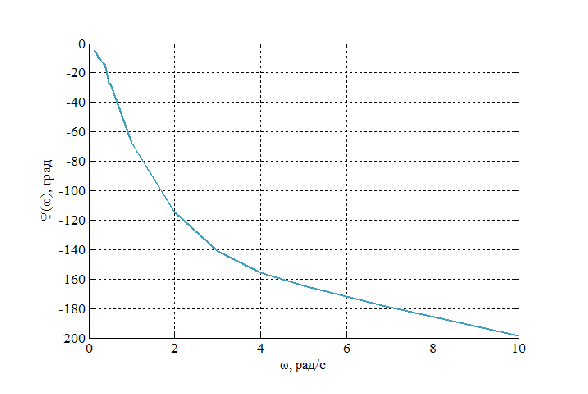
\includegraphics[width=1\linewidth]{scheme/Fch2.eps}
	\caption{ФЧХ}
\end{figure}
\begin{figure}[H]
	\centering
	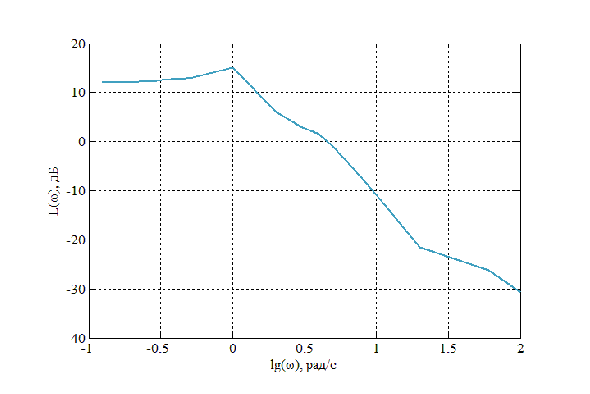
\includegraphics[width=1\linewidth]{scheme/Lach2.eps}
	\caption{ЛАЧХ}
\end{figure}
\begin{figure}[H]
	\centering
	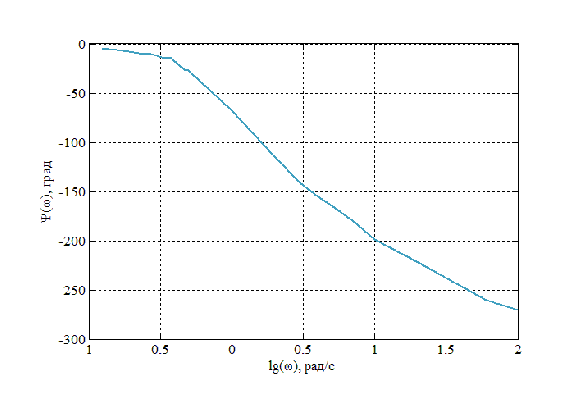
\includegraphics[width=1\linewidth]{scheme/Lfch2.eps}
	\caption{ЛФЧХ}
\end{figure}
\begin{figure}[H]
	\centering
	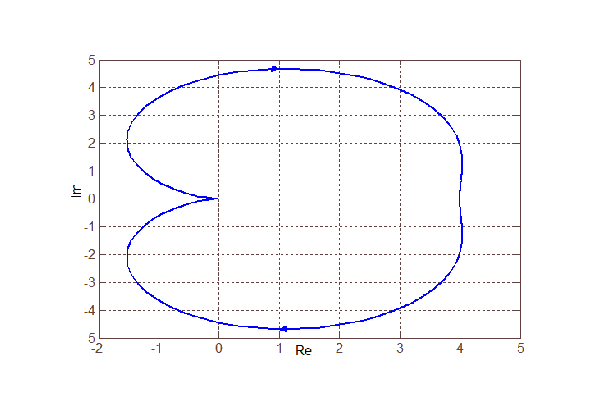
\includegraphics[width=1\linewidth]{scheme/Afch2.eps}
	\caption{АФЧХ}
\end{figure}
\begin{figure}[H]
	\centering
	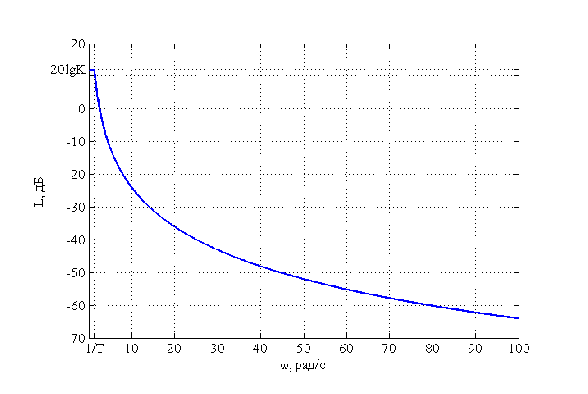
\includegraphics[width=1\linewidth]{scheme/Asi2.eps}
	\caption{Асимптотическая ЛАЧХ}
\end{figure}

\newpage
\begin{center}
\section{Изодромное звено}
\end{center}

В таблице 4 представлены данные при исследовании изодромного звена.
\begin{table}[h!]
	\renewcommand{\arraystretch}{1.8} %строки
	\centering
	\begin{threeparttable}
		\caption{Экспериментальные данные для изодромного звена}
		\begin{tabular}{|c|c|c|c|c|}
			\hline $\omega$, рад/с & $lg\omega$ & $A(\omega)$ & $L(\omega)=20lgA(\omega)$ & $\psi(\omega)$, град\\
			\hline 0,125 & -0,90 & 64,15 & 36,14 & -4,8\\
			\hline 0,175 & -0,75 & 45,94 & 33,24 & -6,67\\
			\hline 0,225 & -0,64 & 35,84 & 31,08 & -9,98\\
			\hline 0,275 & -0,56 & 29,44 & 29,37 & -10,61\\
			\hline 0,325 & -0,48 & 25,02 & 27,96 & -13,65\\
			\hline 0,375 & 0,42 & 21,80 & 26,76 & -14,18\\
			\hline 0,425 & 0,37 & 19,35 & 25,73 & -21,16\\
			\hline 0,475 & 0,32 & 17,43 & 24,82 & -26,92\\
			\hline 0,500 & 0,30 & 16,06 & 24,11 & -27,36\\
			\hline 1,000 & 0,00 & 9,11 & 19,19 & -67,72\\
			\hline 2,000 & 0,30 & 5,77 & 15,22 & -114,36\\
			\hline 3,000 & 0,47 & 4,80 & 13,62 & -140,95\\
			\hline 4,000 & 0,60 & 4,35 & 12,77 & -155,61\\
			\hline 5,000 & 0,69 & 4,09 & 12,25 & -164,73\\
			\hline 7,000 & 0,84 & 3,88 & 11,78 & -179,28\\
			\hline 10,000 & 1,00 & 3,62 & 11,18 & -198,82\\			
			\hline 20,000 & 1,30 & 3,40 & 10,64 & -222,31\\			
			\hline 60,000 & 1,77 & 3,26 & 10,28 & -260,00\\			
			\hline 100,000 & 2,00 & 3,24 & 10,21 & 270,00\\
			\hline
		\end{tabular}
	\end{threeparttable}
\end{table}

На рисунках 14-19 представлены частотные характеристики изодромного звена.
\begin{figure}[H]
	\centering
	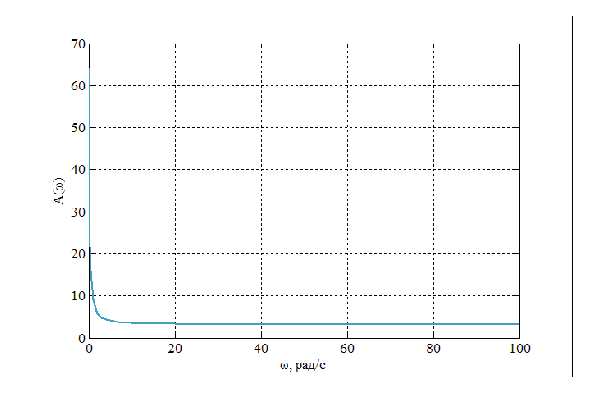
\includegraphics[width=1\linewidth]{scheme/Ach3.eps}
	\caption{АЧХ}
\end{figure}
\begin{figure}[H]
	\centering
	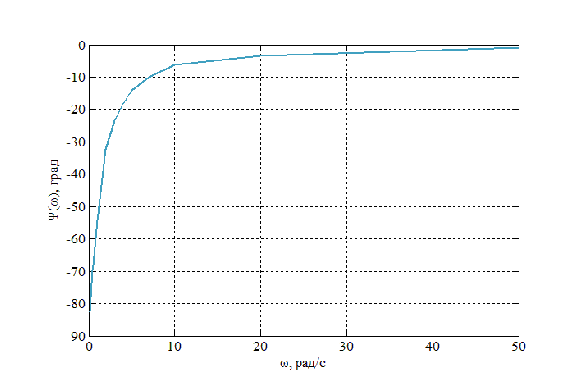
\includegraphics[width=1\linewidth]{scheme/Fch3.eps}
	\caption{ФЧХ}
\end{figure}
\begin{figure}[H]
	\centering
	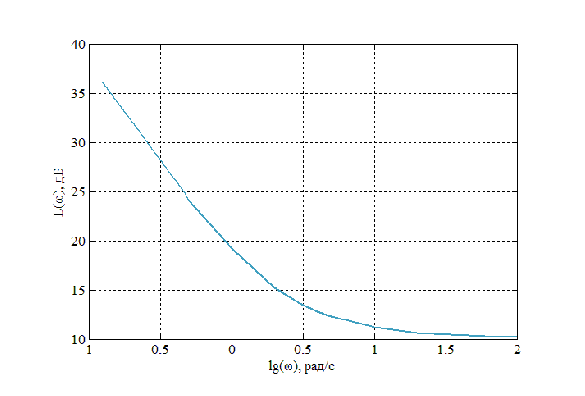
\includegraphics[width=1\linewidth]{scheme/Lach3.eps}
	\caption{ЛАЧХ}
\end{figure}
\begin{figure}[H]
	\centering
	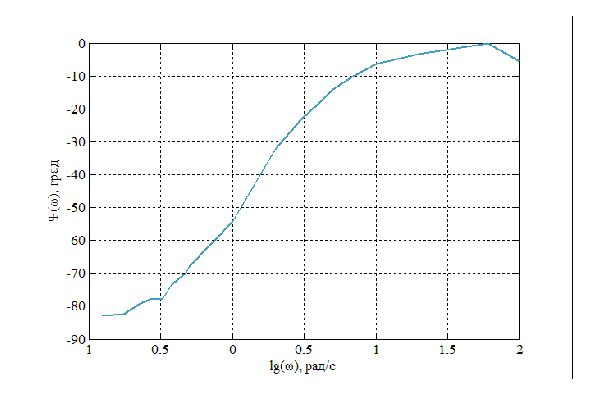
\includegraphics[width=1\linewidth]{scheme/Lfch3.eps}
	\caption{ЛФЧХ}
\end{figure}
\begin{figure}[H]
	\centering
	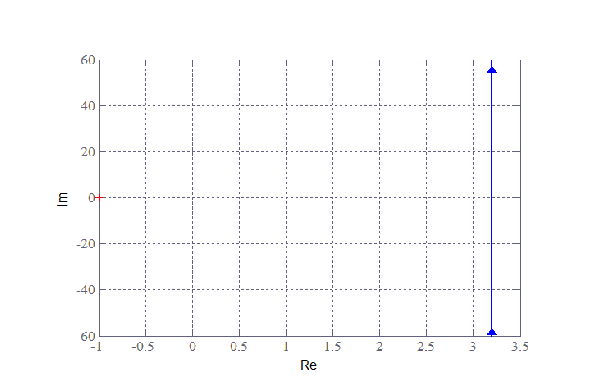
\includegraphics[width=1\linewidth]{scheme/Afch3.eps}
	\caption{АФЧХ}
\end{figure}
\begin{figure}[H]
	\centering
	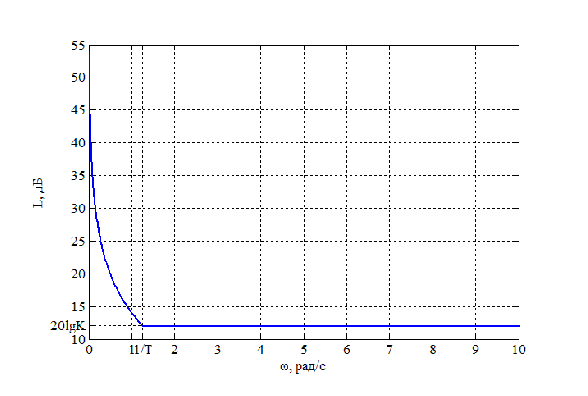
\includegraphics[width=1\linewidth]{scheme/Asi3.eps}
	\caption{Асимптотическая ЛАЧХ}
\end{figure}

\newpage
\begin{center}
	\section*{Вывод}
\end{center}
\par
В ходе лабораторной работы были изучены частотные и логарифмические частотные характеристики типовых динамических звеньев: апериодического 1-го порядка, колебательного и изодромного.
Основываясь на данных можно говорить о том, что фазовый сдвиг для колебательного звена изменяется в пределах от $0^{\circ}$ до $-180^{\circ}$, для изодромного от $-90^{\circ}$ до $0^{\circ}$, а для апериодического звена 1-го порядка фазовый сдвиг от $-90^{\circ}$ до $0^{\circ}$.\par
Сравнивая графики ЛАЧХ и асимптотической ЛАЧХ, можно заметить, что асимптотические ЛАЧХ сходятся к реальным ЛАЧХ, и с их помощью удобно проводить синтез систем управления.\par
Также можно сделать вывод о том, что асимптотическая ЛАЧХ меняет свой наклон при частоте среза $\omega_c = 1/T$ и для её построения не требуется выполнения дополнительных вычислений, достаточно лишь знать вид передаточной функции.Также по асимптотический ЛАЧХ можно восстановить передаточную функцию.  
\end{document}